
\begin{exercice}[]
Calcule le périmètre et l'aire de la plaque métallique représentée ci‑dessous.

\begin{center}
    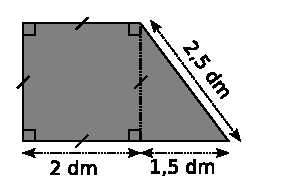
\includegraphics[width=.5\linewidth]{eaCD01}
\end{center}
\end{exercice}



\begin{exercice}[]
La figure suivante représente un morceau de tissu. Calcule son aire.
\begin{center}
    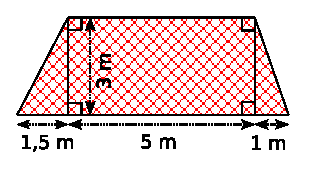
\includegraphics[width=.66\linewidth]{eaCD02}
\end{center}
\end{exercice}

\begin{exercice}[]
On souhaite entourer, avec du grillage, un jardin carré de 24\,m de côté, en laissant une ouverture de 4\,m de large. Le grillage choisi coûte 15\,€ le mètre. Quel sera le prix à payer ?
\end{exercice}

\begin{exercice}[]
M. Albert vend un terrain représenté ci‑dessous, au prix de 18\,€ le m\up{2}.

\begin{center}
    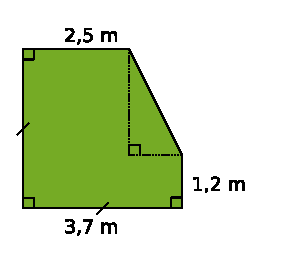
\includegraphics[width=.4\linewidth]{eaCD03}
\end{center}

Quel est le prix de vente de ce terrain ?
\end{exercice}

\begin{exercice}[]
Donne une valeur approchée au dixième du périmètre et de l'aire de la figure.

\begin{center}
    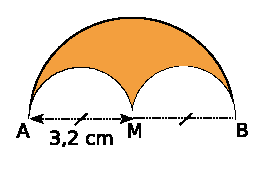
\includegraphics[width=.5\linewidth]{eaCD04}
\end{center}
\end{exercice}

\begin{exercice}[]
Donne la valeur approchée par excès à l'unité du périmètre et de l'aire de la partie jaune.
\begin{center}
    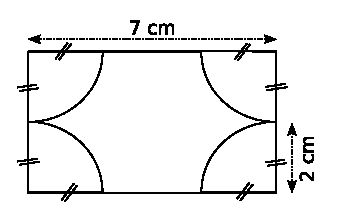
\includegraphics[width=.7\linewidth]{eaCD05}
\end{center}
\end{exercice}

\begin{exercice}[]
Dans une pièce de bois rectangulaire de dimensions 10,2\,cm sur 6,6\,cm, un menuisier découpe un losange. Il perce ensuite, au centre de ce losange, un trou circulaire de 1\,cm de diamètre.

\begin{center}
    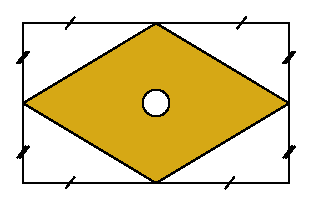
\includegraphics[width=.7\linewidth]{eaCD06}
\end{center}

Donne un arrondi à l'unité de l'aire de la pièce de bois obtenue.
\end{exercice}

\begin{exercice}[]
Un massif circulaire a un diamètre de 10\,m. On souhaite y planter 50 rosiers régulièrement espacés, à 30\,cm du bord. Quelle distance y aura‑t‑il entre chaque plant ? (Donne le résultat arrondi au centimètre.)
\end{exercice}

\begin{exercice}[]
Un artisan rénove une pièce de 3,50\,m de largeur, 4\,m de longueur et 2,50\,m de hauteur. 

\begin{colenumerate}{1} 
\item Sur le plafond, il met deux couches de peinture. Un pot de peinture permet de couvrir 6\,m\up{2}. De combien de pots a-t-il besoin ?
\item Il tapisse tous les murs avec du papier peint. Chaque rouleau est large de 50\,cm et long de 10\,m, sans raccord. Combien de rouleaux doit-il prévoir ? On ne tiendra pas compte des ouvertures (portes et fenêtres).
\end{colenumerate} 
\end{exercice}

\begin{exercice}[]
Construis un parallélogramme qui a un côté de 6\,cm de longueur, un périmètre de 20\,cm et une aire de 18\,cm\up{2}. Justifie ta construction en indiquant tes calculs.
\end{exercice}

\begin{exercice}[Attention travaux !]
Un peintre en bâtiment fait l’expérience suivante : il imbibe entièrement son rouleau de peinture, il le pose sur le mur, le fait rouler en lui faisant faire seulement un tour complet, puis le retire du mur.

\begin{colenumerate}{1} 
\item Quelle va être la forme de la tache de peinture ainsi réalisée ?
\item Le rouleau est large de 25\,cm et d’un diamètre de 8\,cm. Quelle surface du mur sera alors recouverte de peinture ?
\item Combien de fois, au minimum, devra-t-il réaliser ce geste pour peindre un mur long de 6\,m et haut de 2,5\,m ?
\end{colenumerate} 
\end{exercice}


\begin{exercice}[La galette]
Un pâtissier doit confectionner une tarte recouverte de glaçage. Il sait qu'avec 100\,g de sucre glace, il fabrique du glaçage pour une surface de 5\,dm\up{2}. Sachant qu'il dispose de moules à tarte circulaires de diamètres 22\,cm, 26\,cm ou 28\,cm, quel moule devra-t-il utiliser pour 100\,g de sucre ?
\end{exercice}

\begin{exercice}[Le nautile]
\ImageDroite{Le nautile est un mollusque dont la coquille est spiralée et peut être schématisée de la manière suivante.}{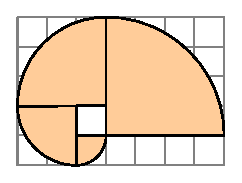
\includegraphics[width=.4\linewidth]{eaCD07}}

\begin{colenumerate}{1} 
\item Reproduis ce schéma dans un quadrillage à carreaux de 1\,cm de côté.
\item Calcule l'aire de la figure.
\item Calcule le périmètre de cette figure.
\end{colenumerate} 
\end{exercice}



\begin{exercice}[Une couronne pour un roi]
\ImageDroite{Calcule l'aire de la couronne circulaire ci-contre en arrondissant le résultat au mm\up{2} le plus proche.}{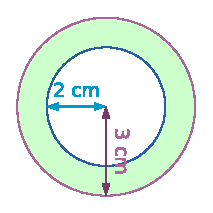
\includegraphics[width=.4\linewidth]{eaCD08}}
\end{exercice}


\begin{exercice}[] 
quadrilatère ABCD est un rectangle tel que $BC = 4$\,cm, $AB = 6$\,cm et $K$ est le milieu de $[AD]$. La surface colorée est formée de parallélogrammes accolés. Montre que l'aire de la surface colorée est la moitié de celle du rectangle.
\begin{center}
    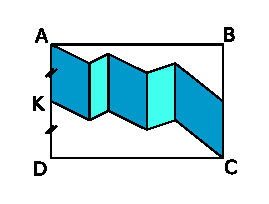
\includegraphics[width=.5\linewidth]{eaCD09}
\end{center}
\end{exercice}

\begin{exercice}[Pare-brise]
Sur un pare-brise rectangulaire de 1,50\,m par 0,80\,m est fixé (au milieu de la longueur) un essuie-glace de longueur 0,65\,m. Trouve une valeur approchée du pourcentage de la surface balayée par rapport à celle du pare-brise.
\end{exercice}


\begin{exercice}
\ImageDroite{On considère un cercle de rayon $r$\,cm ($r > 0$).}{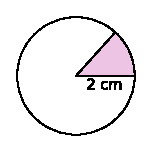
\includegraphics[width=.25\linewidth]{eaCD10}}

\begin{colenumerate}{1} 
\item\label{CDea1} On suppose ici que $r = 2$. Calcule l'aire de chaque secteur circulaire dont l'angle est donné dans le tableau suivant.

\vspace{1em}

% la commande de centrage des colonnes provoquent des erreurs ici
%\renewcommand*\tabularxcolumn[1]{>{\centering\arraybackslash}m{#1}}
{\footnotesize
\begin{ltableau}{\linewidth}{5}
\hline
Angle ($\circ$) & 360 & 90 & 45 & 180  \\ \hline
Aire (cm\up{2}) & & & &  \\ \hline
\end{ltableau}

\vspace{.5em}

\begin{ltableau}{\linewidth}{9}
\hline
Angle ($\circ$) & 120 & 3 & 1 & 12 \\ \hline
Aire (cm\up{2}) & & & & \\ \hline
\end{ltableau}
}% fin du footnotesize

\item Calcule le coefficient de proportionnalité du tableau précédent.
\item\label{CDea3} À l'aide du \ref{CDea1}, établis la formule donnant l'aire du secteur angulaire ci-dessous en faisant intervenir $x$, $r$ et le nombre $\pi$.

\begin{center}
    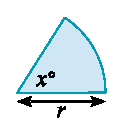
\includegraphics[width=.25\linewidth]{eaCD11}
\end{center}

\item\label{CDea4} En utilisant la formule établie à la question \ref{CDea3}, calcule l'aire exacte des figures suivantes.

    \begin{center}
        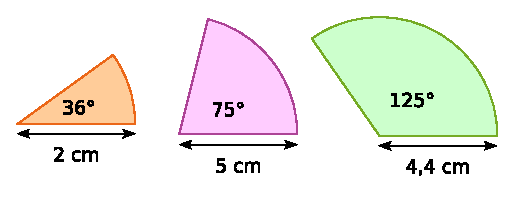
\includegraphics[width=\linewidth]{eaCD12}
    \end{center}
\item Déduis de la question \ref{CDea4} l'aire exacte :
    \subitem \textbullet d'un secteur angulaire de rayon 1\,cm et d'angle 111$^\circ$ ;
    \subitem \textbullet d'un secteur angulaire de rayon 8\,cm et d'angle 50$^\circ$.
\end{colenumerate} 
\end{exercice}


\begin{exercice}[Œuf de Pâques]
Voici un œuf de Pâques construit sur du papier pointé. L'unité est le centimètre. Le segment $[AO]$ mesure 4\,cm.

\begin{center}
    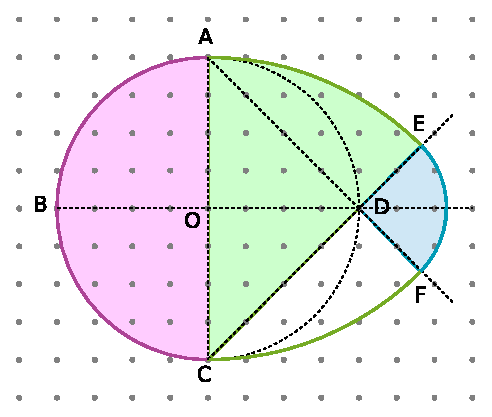
\includegraphics[width=\linewidth]{eaCD13}
\end{center}

\begin{center}\textbf{Construction}\end{center}

\begin{colenumerate}{1} 
\item Reproduis cette figure sur ton cahier. 
\item Propose un programme de construction pour cette figure.

\begin{center}\textbf{Les différentes parties de l'œuf}\end{center}

\item Cherche le rayon du demi-disque rose puis calcule son aire.
\item Cherche le rayon du huitième de disque vert puis calcule son aire.
\item Le segment $[AD]$ mesure 5,7\,cm. Cherche la longueur du segment $[DF]$ puis calcule l'aire du quart de disque bleu. 

\begin{center}\textbf{Aire de l'œuf}\end{center}


\item Un élève dit : \og Pour calculer l’aire de l'œuf, j’additionne l’aire de la partie rose, celle de la partie bleue et deux fois celle de la partie verte. \fg. A-t-il raison ? Sinon, explique.
\item Calcule l'aire du triangle rectangle $ADC$. 
\item Calcule alors une valeur approchée au dixième de l’aire de l'œuf.
 
\begin{center}\textbf{Un joli ruban}\end{center}

Marion veut entourer son œuf d'un joli ruban de laine en suivant le tour de l'œuf $AEFCBA$. 
\item Calcule une valeur approchée au dixième de la longueur de ruban nécessaire pour parer l'œuf de ce joli ruban.
\end{colenumerate} 
\end{exercice}

\begin{exercice}[]
Dans chaque cas, construis tous les quadrilatères qui satisfont aux énigmes suivantes.

\begin{colenumerate}{1} 
\item Je suis un quadrilatère dont les angles opposés sont égaux deux à deux. Mon aire vaut 28\,cm\up{2} et mon périmètre 24\,cm. Mes côtés ont des mesures entières.
\item Je suis un parallélogramme dont les diagonales sont de même longueur. La connaissance soit de la longueur d’une diagonale, soit d’un de mes côtés suffit pour que l’on puisse calculer mon aire qui est égale à 8\,cm\up{2}.
\item Je suis un quadrilatère non croisé qui a deux côtés consécutifs égaux et qui possède ses diagonales perpendiculaires. Mon aire vaut 24\,cm\up{2}. Mes diagonales ont des mesures entières et mon centre se trouve au quart de la plus grande diagonale.
\end{colenumerate}
\end{exercice}
